\documentclass[border=2pt,draw]{standalone}
\usepackage{tikz}
\usetikzlibrary{fit}
\begin{document}

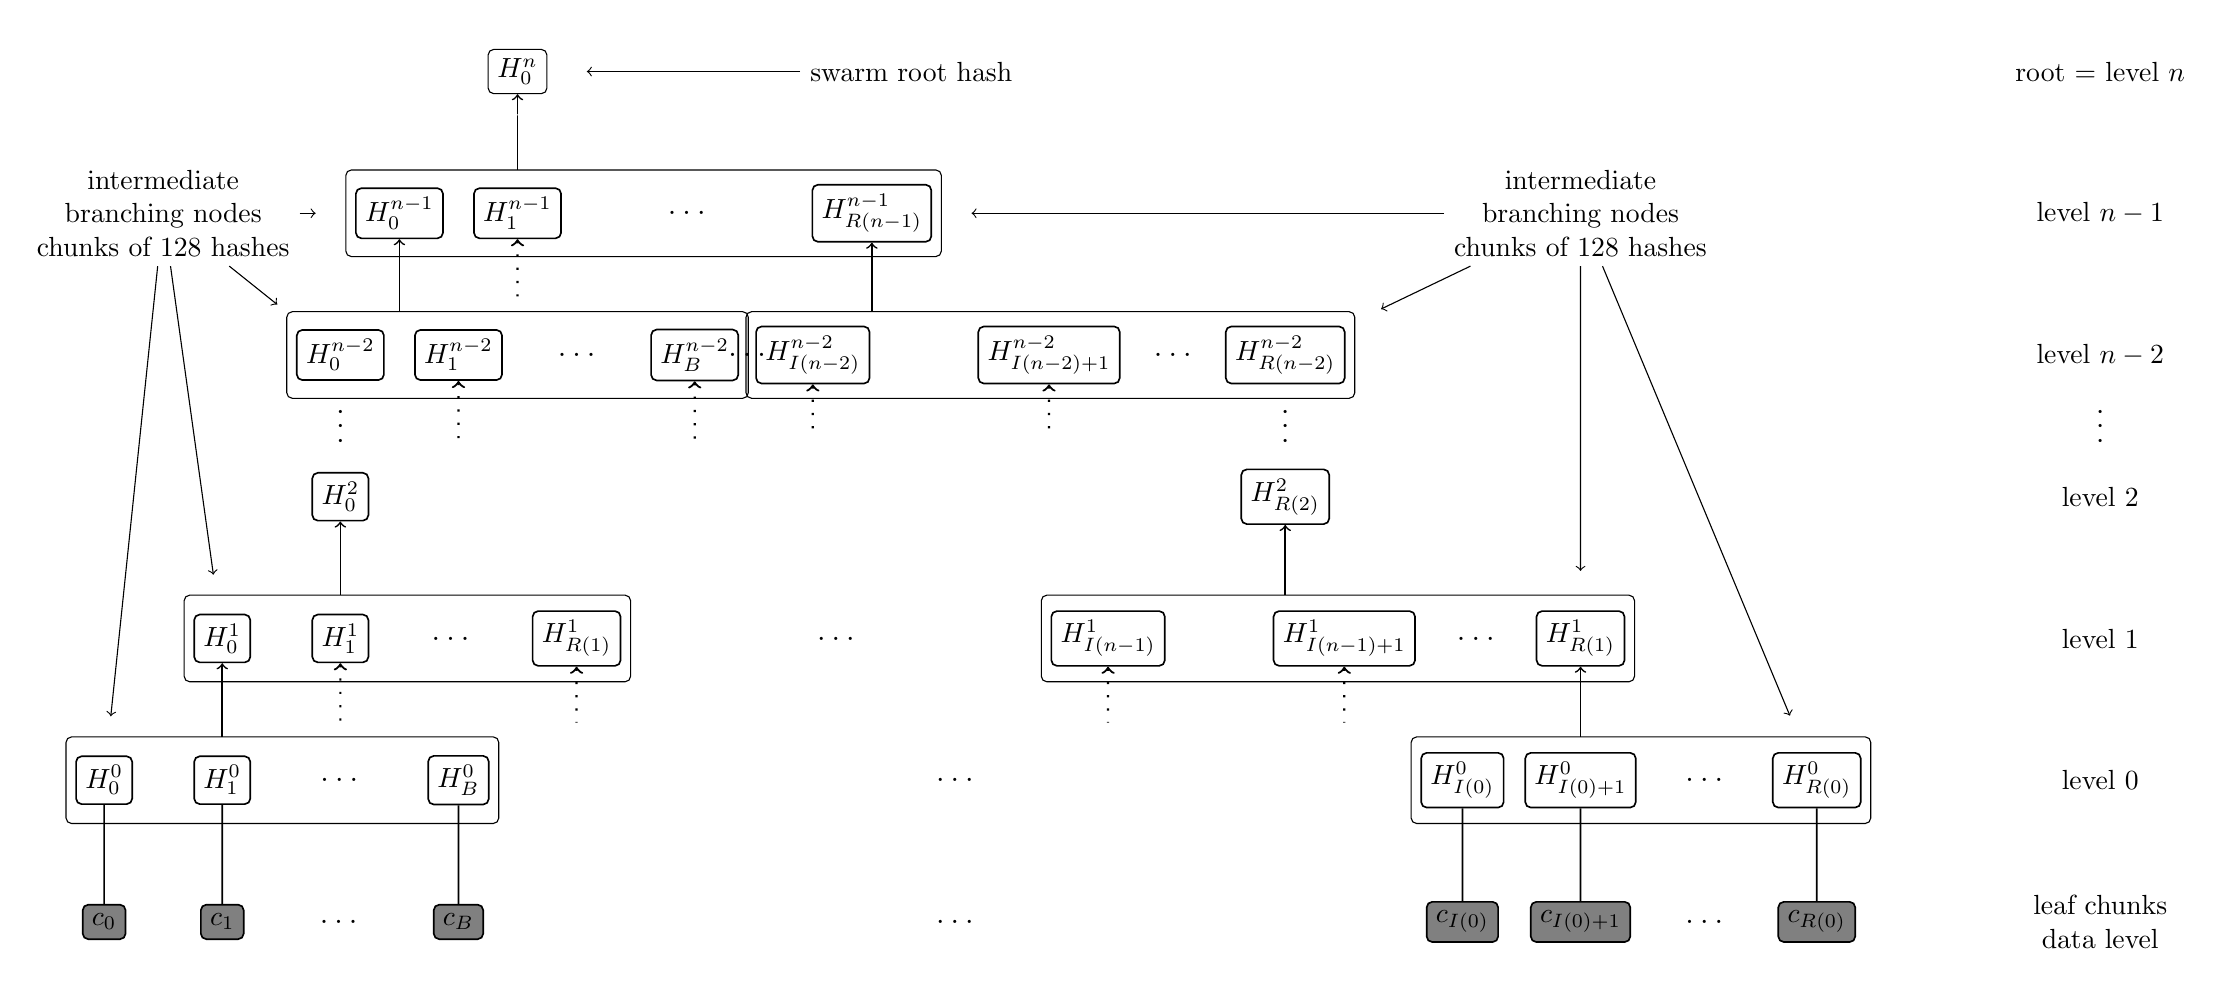
\begin{tikzpicture}[level/.style={sibling distance=15mm, line width=0.6pt, level distance=18mm},
]
\node [rounded corners=2pt,draw] (root) {$H^n_0$}
  child[grow=down,draw=none] { node {} edge from parent[<-,shorten >=12pt]}
  child[grow=right,draw=none,level distance=5cm] { node (swh) {swarm root hash} edge from parent[draw=none] }
  child {node [rounded corners=2pt,draw] (n-10) {$H^{n-1}_{0}$} edge from parent[draw=none]
    child[grow=down,draw=none] { node {} edge from parent[<-, shorten >=12pt]}
    child[grow=left,draw=none,level distance=3cm] { node[align=center] (bnl) {intermediate\\branching nodes\\chunks of 128 hashes}  edge from parent[draw=none] }
    child {node [rounded corners=2pt, draw] (n-2l0) {$H^{n-2}_{0}$} edge from parent[draw=none]
      child {node [rounded corners=2pt, draw] (2l0) {$H^{2}_{0}$} edge from parent[draw=none]
        child[grow=down,draw=none] { node {} edge from parent[<-, shorten >=12pt]}
        child {node [rounded corners=2pt, draw] (1l0) {$H^{1}_{0}$} edge from parent[draw=none]
          child[grow=down,draw=none] { node {} edge from parent[<-, shorten >=12pt]}
          child {node [rounded corners=2pt,draw] (0l0) {$H^{0}_{0}$} edge from parent[draw=none]
            child {node [fill=gray, rounded corners=2pt,draw] {$c_{0}$}}
          }
          child {node [rounded corners=2pt,draw] (0l1) {$H^{0}_{1}$} edge from parent[draw=none]
            child {node [fill=gray, rounded corners=2pt,draw] (cl1) {$c_{1}$}}
          }
          child[missing]
          child {node [rounded corners=2pt,draw] (0ll) {$H^{0}_{B}$} edge from parent[draw=none]
            child {node [fill=gray, rounded corners=2pt,draw] (cll) {$c_{B}$}}
          }
        }
        child {node [rounded corners=2pt,draw] (1l1) {$H^{1}_{1}$} edge from parent[draw=none]
          child[thick,loosely dotted, shorten >=6mm, thick,<-] {node {}}
        }
        child[missing]
        child {node [rounded corners=2pt,draw] (1ll) {$H^{1}_{R(1)}$} edge from parent[draw=none]
          child[thick,loosely dotted, shorten >=6mm, thick,<-] {node {}}
        }
      }
    }
    child {node [rounded corners=2pt, draw] (n-2l1) {$H^{n-2}_{1}$} edge from parent[draw=none]
      child[thick,loosely dotted, shorten >=6mm, thick,<-] {node {}}
    }
    child[missing]
    child {node [rounded corners=2pt, draw] (n-2ll) {$H^{n-2}_{B}$} edge from parent[draw=none]
      child[thick,loosely dotted, shorten >=6mm, thick,<-] {node {}}
    }
  }
  % child[missing]
  child {node [rounded corners=2pt,draw] (n-11) {$H^{n-1}_{1}$} edge from parent[draw=none]
    child[thick,loosely dotted, shorten >=6mm, thick,<-] {node {}}
  }
  % child[missing]
  child[missing]
  child[missing]
  child {node [rounded corners=2pt,draw] (n-1l) {$H^{n-1}_{R(n-1)}$} edge from parent[draw=none]
    child[grow=down,draw=none] { node {} edge from parent[<-, shorten >=12pt]}
    child[grow=right,level distance=9cm] { node[align=center] (bnr)  {intermediate\\branching nodes\\chunks of 128 hashes} edge from parent[draw=none]}
    child[missing]
    child {node [rounded corners=2pt, draw] (n-2r0) {$H^{n-2}_{I(n-2)}$} edge from parent[draw=none]
      child[thick,loosely dotted, shorten >=6mm, thick,<-] {node {}}
    }
    child[missing]
    child {node [rounded corners=2pt, draw] (n-2r1) {$H^{n-2}_{I(n-2)+1}$} edge from parent[draw=none]
      child[thick,loosely dotted, shorten >=6mm, thick,<-] {node {}}
    }
    % child[missing]
    child[missing]
    child {node [rounded corners=2pt, draw] (n-2rl) {$H^{n-2}_{R(n-2)}$} edge from parent[draw=none]
      child[grow=down] {node [rounded corners=2pt, draw] (2rl) {$H^{2}_{R(2)}$} edge from parent[draw=none]
      child[grow=down,draw=none] { node {} edge from parent[<-, shorten >=12pt]}
        child {node [rounded corners=2pt, draw] (1r0) {$H^{1}_{I(n-1)}$} edge from parent[draw=none]
          child[thick,loosely dotted, shorten >=6mm, thick,<-] {node {}}
        }
        child[missing]
        child {node [rounded corners=2pt,draw] (1r1) {$H^{1}_{I(n-1)+1}$} edge from parent[draw=none]
          child[thick,loosely dotted, shorten >=6mm, thick,<-] {node {}}
        }
        % child[missing]
        child[missing]
        child {node [rounded corners=2pt,draw] (1rl) {$H^{1}_{R(1)}$} edge from parent[draw=none]
          child[grow=down,draw=none] { node {} edge from parent[<-, shorten >=12pt]}
          child {node [rounded corners=2pt,draw] (0r0) {$H^{0}_{I(0)}$} edge from parent[draw=none]
            child {node [fill=gray, rounded corners=2pt,draw] (cr0) {$c_{I(0)}$}}
          }
          child {node [rounded corners=2pt,draw] (0r1) {$H^{0}_{I(0)+1}$} edge from parent[draw=none]
            child {node [fill=gray, rounded corners=2pt,draw] (cr1) {$c_{I(0)+1}$}}
          }
          child[missing]
          child {node [rounded corners=2pt,draw] (0rl) {$H^{0}_{R(0)}$} edge from parent[draw=none]
            child {node [fill=gray, rounded corners=2pt,draw] (crl) {$c_{R(0)}$}
              child [grow=right] { edge from parent[draw=none]
                child [grow=right] {node[align=center] {leaf chunks\\data level} edge from parent[draw=none]
                  child [grow=up] {node {level $0$} edge from parent[draw=none]
                    child [grow=up] {node {level $1$} edge from parent[draw=none]
                      child [grow=up] {node (l2) {level $2$} edge from parent[draw=none]
                        child [grow=up] {node (ln-2) {level $n-2$} edge from parent[draw=none]
                          child [grow=up] {node {level $n-1$} edge from parent[draw=none]
                            child [grow=up] {node {root = level $n$} edge from parent[draw=none]}
                          }
                        }
                      }
                    }
                  }
                }
              }
            }
          }
        }
      }
    }
  };

\path (n-11) -- (n-1l) node [midway,font=\large] {$\ldots$};
\path (n-2l0) -- (2l0) node [midway,font=\large,sloped] {$\ldots$};
\path (n-2rl) -- (2rl) node [midway,font=\large,sloped] {$\ldots$};
\path (ln-2) -- (l2) node [midway,font=\large,sloped] {$\ldots$};
\path (1l1) -- (1ll) node [midway,font=\large] {$\ldots$};
\path (1r1) -- (1rl) node [midway,font=\large] {$\ldots$};
\path (1ll) -- (1r0) node [midway,font=\large] {$\ldots$};
\path (n-2l1) -- (n-2ll) node [midway,font=\large] {$\ldots$};
\path (n-2r1) -- (n-2rl) node [midway,font=\large] {$\ldots$};
\path (n-2ll) -- (n-2r0) node [midway,font=\large,sloped] {$\ldots$};
\path (0l1) -- (0ll) node [midway,font=\large] {$\ldots$};
\path (0r1) -- (0rl) node [midway,font=\large] {$\ldots$};
\path (0ll) -- (0r0) node [midway,font=\large] {$\ldots$};
\path (cl1) -- (cll) node [midway,font=\large] {$\ldots$};
\path (cr1) -- (crl) node [midway,font=\large] {$\ldots$};
\path (cll) -- (cr0) node [midway,font=\large] {$\ldots$};

\begin{scope}[shorten >=.5cm,thin]
\draw [->] (swh) -> (root);
\draw [->] (bnl) -> (n-10);
\draw [->] (bnl) -> (n-2l0);
\draw [->] (bnl) -> (1l0);
\draw [->] (bnl) -> (0l0);
\draw [->] (bnr) -> (n-1l);
\draw [->] (bnr) -> (n-2rl);
\draw [->] (bnr) -> (1rl);
\draw [->] (bnr) -> (0rl);
\end{scope}

\node[rounded corners=2pt, draw=white, minimum height=1.1cm, fit=(root)] {};
\node[rounded corners=2pt, draw=black, minimum height=1.1cm, fit=(0l0) (0ll)] {};
\node[rounded corners=2pt, draw=black, minimum height=1.1cm, fit=(n-2l0) (n-2ll)] {};
\node[rounded corners=2pt, draw=black, minimum height=1.1cm, fit=(n-2r0) (n-2rl)] {};
\node[rounded corners=2pt, draw=black, minimum height=1.1cm, fit=(1l0) (1ll)] {};
\node[rounded corners=2pt, draw=black, minimum height=1.1cm, fit=(1r0) (1rl)] {};
\node[rounded corners=2pt, draw=black, minimum height=1.1cm, fit=(n-10) (n-1l)] {};
\node[rounded corners=2pt, draw=black, minimum height=1.1cm, fit=(0r0) (0rl)] {};
\end{tikzpicture}

\end{document}
%R_B(1)+M_B(1)